
\begin{tikzpicture}

% % always
\node (ds) at (5,0){};
\node (dsy) at (5,4){};
\node (dsx) at (10,0){};
\node (lab1) at (1,-1){\textbf{Chemical Space $C_f$}};
\foreach \x in {0,1,2}
		\foreach \y in {1,2,3}{
		\node[rectangle,fill=teal,minimum width = 0.05cm] (place\x\y) at (\x,\y){};}
% % two
\visible<2->{\node[draw,circle,very thick,red,minimum width = 0.5cm,label=right:{\color{red}$c_i$}] (ci) at (1,3){};}


% % three
\visible<1->{\node[circle, black,thick,minimum width = 2.7cm,minimum height = 2.7cm,path picture={\node at (path picture bounding box.center){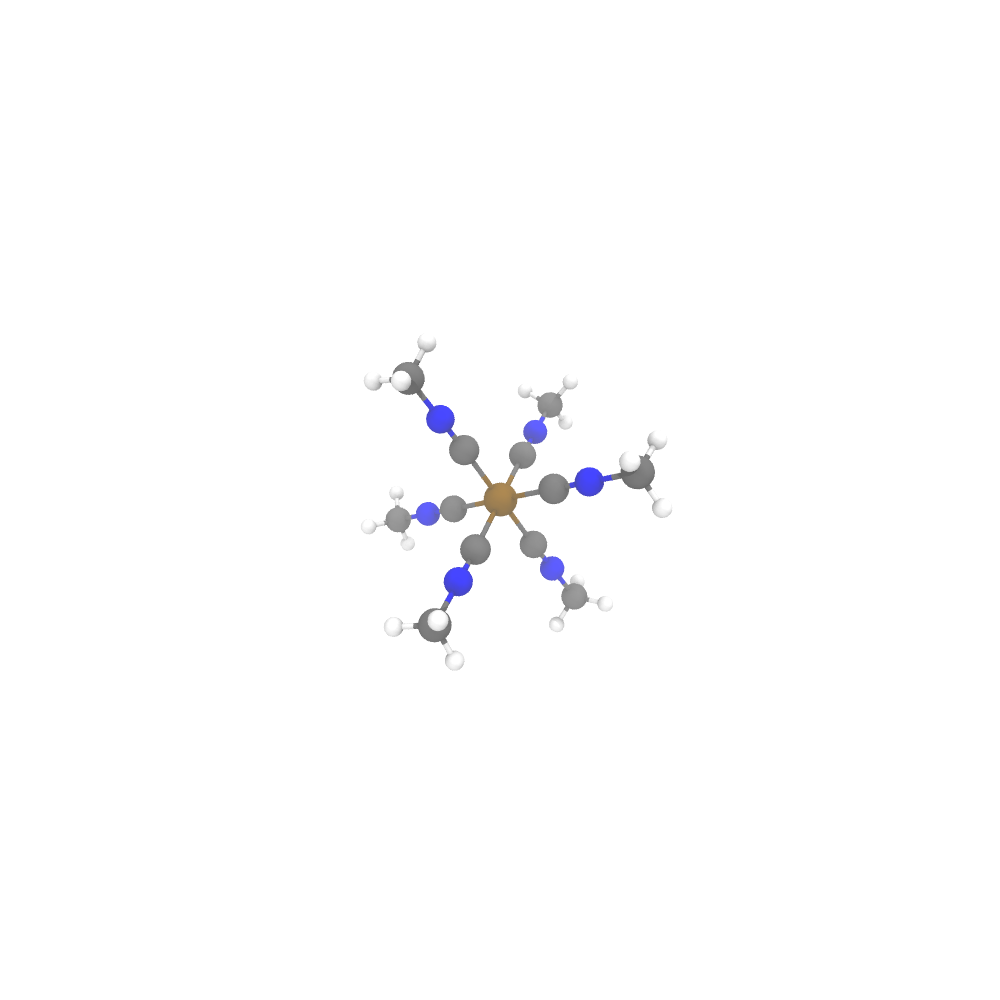
\includegraphics[width=7.5cm]{representations/images/misc}}; }] (Ap) at (3.45,3.75) {};}
\visible<1->{\node (A) at (3.45,3.75) {};}
\visible<1->{\node[draw,circle,very thick,red,minimum width = 2.75cm] (cic) at (3.45,3.75){};}
\visible<1->{\path[draw,red,dashed,very thick] (ci.north) edge node[below] {} (cic.north west);}
\visible<1->{\path[draw,red,dashed,very thick] (ci.south) edge node[below] {} (cic.south);}

% % four
\visible<1->{\path[draw,very thick] (ds.center) -- (dsx);}
\visible<1->{\path[draw,very thick] (ds.center) -- (dsy);}
\visible<1->{\node (lab1) at (7,-1){\textbf{Descriptor Space $\mathcal{X}\subset \mathbb{R}^{d}$}};}

% % five
\visible<1->{\node[circle, fill=black,minimum width =0.05cm,label=below:{$\mathbf{x}_i$}] (x) at (6,3) {};}
\visible<1->{\path[draw, thick,red] (cic.north east) edge[bend left,->] node[above] {} (x);}


% % six
\visible<1->{\node[circle, fill=black,minimum width =0.05cm,label=right:{$\mathbf{x}_{j}$}] (x3) at (8,1) {};}

% % seven
\visible<1->{\node[draw,circle,very thick,red,minimum width = 0.5cm,label=below:{\color{red}$c_j$}] (cj) at (2,1){};}
\visible<1->{\node[circle, black,thick,minimum width = 2.7cm,minimum height = 2.7cm,path picture={\node at (path picture bounding box.center){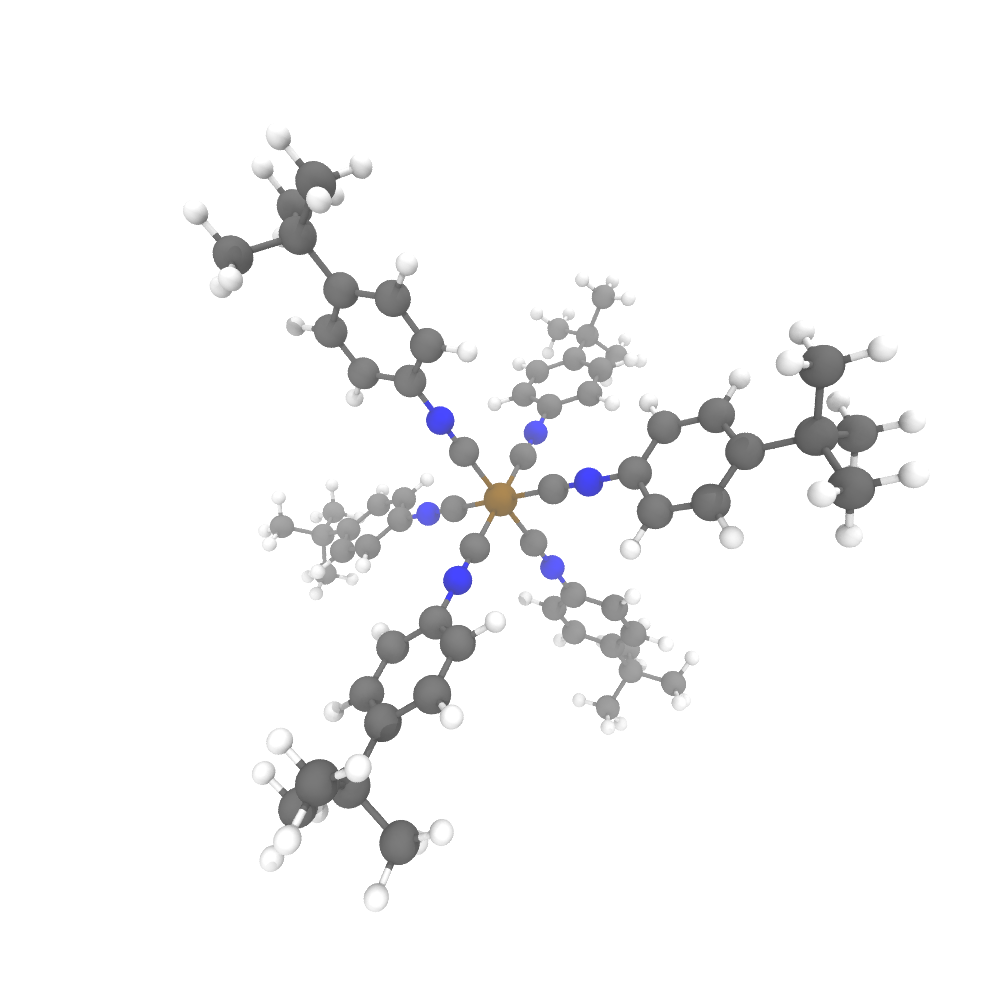
\includegraphics[width=3cm]{representations/images/pisc_trans}}; }] (Xp) at (4.2,0.75) {};}
\visible<1->{\node[draw,circle,very thick,red,minimum width = 2.75cm] (cicj) at (4.2,0.75){};}
\visible<1->{\path[draw,red,dashed,very thick] (cj.north) edge node[below] {} (cicj.north west);}
\visible<1->{\path[draw,red,dashed,very thick] (cj.south) edge node[below] {} (cicj.south west);}
\visible<1->{\path[draw, thick,red] (cicj.south east) edge[bend right,->] node[below] {} (x3);}

% % eight
\visible<1->{\path[draw,dashed,gray,very thick,|-|] (x) -- (x3);}
\visible<1->{\node[gray] (ddist) at (8,2){$d(\mathbf{x}_i,\mathbf{x}_j)$};}

% %
\visible<1->{\node[align=left] (gd) at (8.2,4) {Good descriptors: \\$\bullet$ cheap \\ $\bullet$ small as possible \\ $\bullet$ preserve similarity};}


\end{tikzpicture}
